\subsubsection{Introduzione}

Con questo firmware si vuole implementare una parte del progetto \textit{Alterline}, che mira a fornire un controllo remoto delle colorazioni delle vetrine di un negozio, con possibilit\`a di essere esteso con nuove funzionalit\`a e di essere il pi\`u possibile automatizzato nella diagnosi degli errori. All'interno del negozio ogni vetrina avr\`a un led RGB, controllato con PWM da una schedina STM32, ognuna di queste schede sar\`a in contatto bluetooth con una scheda centrale (per cui questo firmware \`e pensato), unica per ogni negozio, che sar\`a a sua volta connessa via ethernet ad un server web, contenente il database utilizzato nel progetto.

\subsubsection{Ambiente di sviluppo}

Il progetto \`e portato avanti sull'IDE \texttt{Atollic TrueStudio for STM32}, partendo da un progetto generato dal software \texttt{STM32CubeMX}, per includere tutte le estensioni Driver e Middelware fornite da ST e poterle configurare in un'unica schermata. Per il controllo delle versioni si ricorre a \texttt{git}, direttamente accessibile da TrueStudio attraverso l'apposita estensione di Eclipse (su cui si basa il tool), \`e cos\`i possibile avere una traccia puntuale dei progressi (attraverso lo storico dei commit) ed \`e possibile creare pi\`u varianti di test del progetto (attraverso i branch).

Il debug pu\`o essere portato avanto con gdb sempre su Atollic, nella Perspective di debug appare anche una finestra con la console SWV dove, se abilitato tramite la flag \texttt{DEBUG} in \texttt{includes/debug.h}, appaiono i log lanciati con PRINTF. In alternativa pu\`o essere utilizzato il software \texttt{STMStudio} per tenere traccia del valore delle variabili durante l'esecuzione (non \`e possibile usare entrambi i metodi contemporaneamente).

\subsubsection{Multithreading con FreeRTOS}

Il progetto implementa le due connettivit\`a (ethernet e bluetooth) in thread separate, all'interno di queste viene eseguita un'azione tra INIT, READ, WRITE o END a seconda del valore della variabile \texttt{*\_state} (presente sia per eth che per ble), che permette di eseguire un operazione per ogni ciclo e passare all'attivit\`a successiva al termine di ciascuna. Una terza thread pu\`o innescare ciascuna trasmissione settando lo stato come INIT (ora viene gestito alla pressione del pulsante).

\subsubsection{Implementazione del database locale}

files \textit{Src/db\_struct.c}, \textit{Inc/db\_struct.h}

Il database interno, per quanto riguarda la comunicazione con il server web, contiene due \texttt{struct}, rispettivamente per i dati del negozio e quelli delle vetrine (array), entrambi hanno 2 istanze statiche e 2 puntatori, \texttt{shadow\_} e \texttt{active\_} (che puntano rispettivamente a una delle due versioni) durante il fetch i dati vengono salvati all'interno delle strutture puntate da \texttt{shadow\_} e se i dati sono coerenti i puntatori \texttt{shadow\_} e \texttt{active\_} vengono scambiati. Alla ricezione della linea riguardante il negozio, vengono controllati l'id e la versione, se il primo coincide e la seconda \`e maggiore di quella salvata localmente, il fetch delle vetrine prosegue. Ogni riga (negozio e vetrina) contiene un checksum calcolato con l'algoritmo BSD su 2 byte, se la sua verifica fallisce il fetch \`e interrotto.

I dati ricevuti dal server web vengono trasferiti dalla struttura \texttt{active\_} alle rispettive vetrine, l\`i saranno gestiti in una tabella pronti per essere attivati in base alla data. Ora \`e possibile la lettura dei dati effettivamente attivi su ciascuna vetrina, che verranno poi salvati in una tabella specifica, contenente anche dati relativi al negozio (\texttt{running\_shop} e \texttt{running\_entries}). Quando tutti i dati sono pronti \`e possibile spedirli al server. Anche l\`i verr\`a controllato il checksum dei dati ricevuti e nel responso sar\`a utilizzato il codice 206 (al posto di 200) per chiedere una ritrasmissione, discorso analogo quando si verifica un errore nel database, qui il codice sar\`a 205. Nel caso di \texttt{shop\_id} errato viene restituito 404 (NOT FOUND) e la scrittura si blocca.

Le tabelle (array di tipo \texttt{struct vetrina}), contengono i dati nell'ordine in cui vengono ricevuti dal server (non necessariamente ordinati) senza lasciare spazi vuoti, viene quindi utilizzata la funzione \texttt{findEntry(id)} che restituisce l'indice corrispondente alla vetrina con id passato come parametro, se presente. Per come \`e costruita, se viene raggiunto un id nullo la tabella \`e giunta al termine. La scrittura dei dati ricevuti dai dispositivi ble segue l'ordinamento imposto dal server (usando quindi findEntries che tiene come riferimento \texttt{active\_entries}), cos\`i facendo se una vetrina presente sul server non pu\`o essere raggiunta, la sua riga nella tabella \texttt{running\_entries} viene segnata con id=0.

Le funzioni di trasferimento hanno nomi del tipo \texttt{[get/set][Shop/Entry][Eth/Ble]}, dove vengono indicati rispettivamente se devono leggere o scrivere dati, per quale struttura e da che interfaccia, in generale servono per decodificare i dati ricevuti o preparare i dati da inviare.

\subsubsection{Database remoto e interfaccia web}

Il database remoto viene gestito su server apache (o qualunque altra alternativa che supporti php e mysql), nella cartella \texttt{server\_files} sono contenute le pagine che devono stare nella cartella pubblica sul server e gli script di creazione del database. \texttt{index.php} non \`e nient'altro che il form iniziale per accedere (lato utente) alla visualizzazione grafica delle tabelle, che avviene su \texttt{control.php}. All'interno di \texttt{fetchData.php} vengono gestite tutte le richieste di lettura dalla board mentre i file \texttt{write*.php} gestiscono rispettivamente la scrittura su server delle vetrine e dei dati del negozio.

Lo script \texttt{create\_table.sql} contiene le istruzioni per definire le due tabelle (vetrine e negozi), collegate da una foreign key che \`e l'id del negozio. Sono presenti anche tabelle \texttt{feedback\_*} con la stessa struttura di vetrine e shops, che conterranno i dati attivi letti dalle board.

Le tabelle vengono popolate con alcuni dati iniziali e viene creato un utente per gestire l'unico negozio inserito, al momento per il negozio 1, l'utente \`e \texttt{shop1} con \texttt{password1} come chiave (da cambiare), \`e importante per\`o che dal nome utente sia deducibile l'id del negozio (per come \`e ora deve essere l'unico numero all'interno del nome). Per evitare di permettere a ciascun utente di poter accedere all'intero database, si possono creare delle VIEW sulle tabelle, in modo da limitare la visione e gestione dell'utente i alle sole righe con i come \texttt{shop\_id} (l'amministratore non avr\`a queste limitazioni).

Per poter aggiornare i dati delle tabelle o del negozio da questa scheda su server, \`e necessario che le righe in tabella siano gi\`a presenti, per questa ragione, ogni volta che verr\`a inserita un vetrina o un negozio si dovr\`a inserire anche nella tabella \texttt{feedback\_*} (o quantomeno inserire una riga contenente gli id corretti). Questo capita perch\'e l'inserimento \`e consentito solamente all'utente root (l'amministratore), mentre gli utenti specifici di ogni negozio possono soltanto eseguire UPDATE su dati gi\`a esistenti. Per ogni nuovo negozio vanno inoltre creati l'utente e tutte le rispettive VIEWS (4 in totale). (\textbf{TODO} includere queste istruzioni in script specifici) 

All'interno degli script php per la gestione del database sono utilizzati dei prepared statement al posto di istruzioni tradizionali, con la spesa di qualche riga di codice in pi\`u, vengono prodotte istruzioni generali, alla quale vengono sostituiti i dati come variabili al momento dell'esecuzione. Questo in genere migliora notevolmente le prestazioni al livello del database, in quanto non \`e necessario un nuovo parsing ad ogni istruzione che differisce solo per valori numerici dalle precedenti (da valutare l'impatto reale su questa applicazione). Inoltre questo metodo protegge ulteriormente da sql injection in quanto i dati inseriti sono sempre numerici (non possono essere inseriti comandi maligni).

\subsubsection{Stati di esecuzione}

files \textit{Src/main.c}, \textit{Inc/main.h}

Dopo le inizializzazioni di hardware e dati (ancora da definire) il sistema entra in funzione e periodicamente aggiorna i dati (ora questo avviene con la pressione del pulsante). Prima, se necessario (\textbf{TODO} da definire) la data viene sincronizzata (\textit{eth}), successivamente parte il fetch dei dati dal server (\textit{eth}), prima i dati del negozio e poi delle vetrine. Questo processo viene saltato qualora la versione locale sia aggiornata, quando questo arriva al termine parte la scrittura dei nuovi dati su ciascuna vetrina (\textit{ble}), successivamente si pu\`o procedere con la lettura dei dati attivi (\textit{ble}) e la risposta al server con questi dati (\textit{eth}), (si pu\`o mettere in parallelo la comunicazione in entrata e in uscita dal server purch\'e non si utilizzi contemporaneamente la stessa interfaccia, \textit{ble} o \textit{eth}, quando finisce dunque la lettura da entrambi i lati si pu\`o passare alla scrittura). Le definizioni di questi processi avvengono nelle funzioni \texttt{[BLE,ETH]\_Process()}, quando lo stato diventa INIT comincia la connessione, ad ogni esecuzione viene eseguita l'operazione indicata (READ/WRITE/SYNC) e se questa va a buon fine, si passa alla successiva, altrimenti in base all problema riscontrato si ripete il procedimento o si termina il servizio (stato END). (\textbf{TODO} implementare una trasmissione delle informazioni sugli errori al server utilizzando lo stato in \texttt{running\_shop}). 

\begin{figure}
	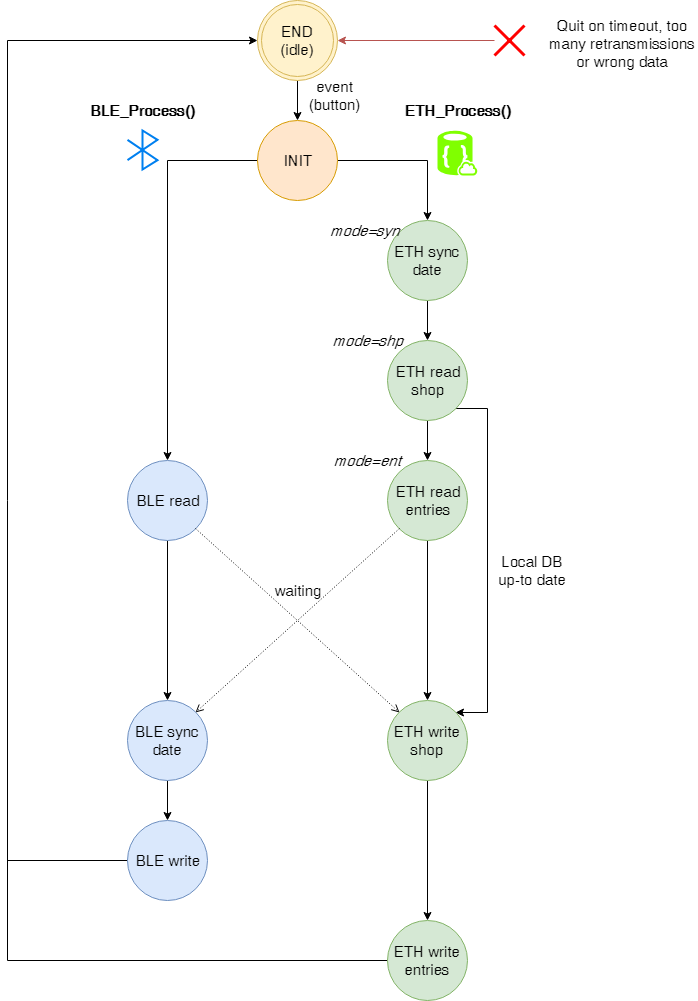
\includegraphics[width=\textwidth]{state_machine}
  \caption{Schema della macchina a stati}
\end{figure}

\begin{figure}
	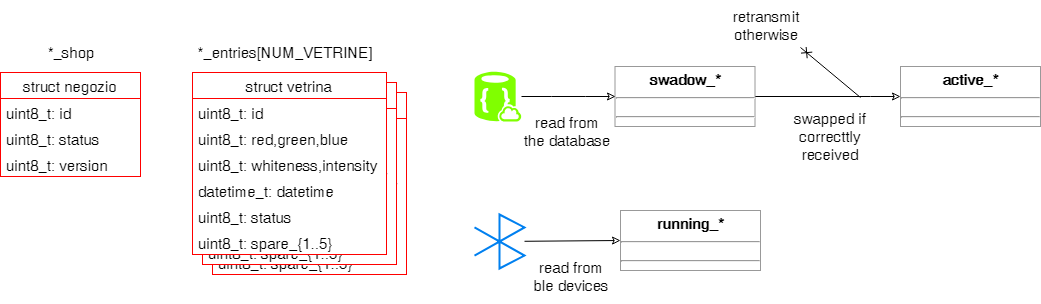
\includegraphics[width=\textwidth]{structures}
  \caption{Struttura del database locale}
\end{figure}

\subsection{COLLEGAMENTO BLUETOOTH STM32F429ZI}

\subsubsection{Comunicazione come client BLE}

funzione \textit{BLE\_Process} e files \textit{Src/sensor\_service.c}, \textit{Inc/sensor\_service.h}

La connessione bluetooth tra master (negozio) e slaves (vetrine) viene gestita utilizzando il primo come client BLE, che richiede letture e scritture sui servizi, detti caratteristiche, forniti dai server (colori, intensit\`a, spare...). L'interazione con ciascuna caratteristica viene fatta in maniera separata ad ogni esecuzione della thread, per fare s\`i che ogni pacchetto sia correttamente ricevuto e gestito. Si interagisce con una vetrina alla volta, vengono dunque eseguite le operazioni su una vetrina, lo stato viene impostato a NEXT e viene chiusa la vecchia connessione per aprirne una nuova con la vetrina successiva. Al termine, per tutte le vetrine, di un'operazione (r/w o sync) si ricomincia dalla prima vetrina con l'operazione seguente. La vetrina che dev'essere utilizzata viene decisa dalle funzioni \texttt{nextEntry()} e \texttt{currEntry()} in \texttt{db\_struct}, che attraverso un indice globale, restituiscono progressivamente gli id delle vetrine presenti in \texttt{active\_table} oppure 0 quando si \`e giunti al termine (e l'indice viene ri-inizializzato). 

Le caratteristiche numeriche vengono convertite in formato testuale, 3 cifre come caratteri ascii per tutte eccetto la data che ne occupa 10 in formato yymmddhhmm. (\textbf{TODO} possibile ottimizzazione accorpando alcune caratteristiche e gestendo pi\`u vetrine in parallelo, se consentito dagli standard)

Durante la lettura/scrittura delle vetrine, vengono usati due array (\texttt{toRead} e \texttt{toWrite}) che contengono gli id dei valori da leggere/scrivere (anche utilizzati come indici per nell'array degli handle), le variabili \texttt{reading} e \texttt{writitng} vengono incrementate ad ogni passo e rappresentano il valore attualmente richiesto al dispositivo ble. Quando queste arrivano al termine (fine dell'array) la procedura \`e terminata e si pu\`o passare alla prossima operazione (per quanto riguarda la lettura esiste una seconda variabile di indice incrementata nel callback all'interno di \texttt{HCI\_Event\_CB}, dove avviene effettivamente la lettura).

Il led blu (LD2) viene attivato all'inizio della comunicazione con la prima vetrina e spento alla fine dell'ultima, per ogni operazione.

\subsection{COLLEGAMENTO ETHERNET STM32F429ZI}

\subsubsection{Crittografia con protocolli TLS/HTTPS}

Per migliorare la sicurezza della comunicazione, il sistema implementa la libreria di cifratura \texttt{mbedtls.h} (selezionabile da STMcube), abbastanza leggera per poter svolgere il suo lavoro con poche risorse e abbastanza avanzata nei metodi e protocolli. La comunicazione HTTP viene dunque 'filtrata' attraverso questa libreria, che la rende dunque accessibile solo a server e client. Durante la procedura di handshake, entrambi gli attori concordano un metodo di cifratura (vengono supportate ciphersuite con \texttt{ECHDE} e certificati \texttt{RSA} o \texttt{ECDSA}, che dovranno essere implementati sul server) e il certificato del server viene controllato (non ne sono stati utilizzati lato client). La scheda \`e in grado di autorizzare certificati self signed solo se il certificato della CA \`e salvato all'interno del firmware (come stringa in \texttt{srv\_cert.c}, \textbf{TODO} implementare un filesystem e caricare l\`i il certificato).

\subsubsection{Comunicazione come client web}

\textsf{funzione \textit{ETH\_Process} e files \textit{Src/mbedtls.c}, \textit{Inc/mbedtls.h}}

Le interazioni (r/w) con il server trattano prima i dati del negozio (id, versione e stato) e successivamente i dati di ciascuna vetrina. Quando la connessione \`e stata stabilita si utilizza la funzione \texttt{PollEthData()} per mandare la richiesta e leggerne il responso, restituendo il corpo del messaggio e eventualmente un codice di errore. 

Le richieste HTTP utilizzano il metodo POST (la query string si trova dentro il corpo del pacchetto) e viaggiano all'interno della stessa connessione TCP creata all'inizio del processo (pressione del bottone) e chiusa quando la comunicazione \`e terminata. La prima richiesta che viene fatta (QUERY \texttt{mode=syn}) richiede dal server data e ora aggiornate (se necessario), successivamente con \texttt{mode=shp} si richiedono i dati specifici del negozio e la versione del database presente sul server, se questi dati sono corretti vengono fatte successive richieste per gli effettivi dati delle vetrine. Questi vengono richiesti con \texttt{mode=ent} e nella risposta il numero di vetrine precede gli altri dati. Nella scrittura su server i dati sono direttamente inclusi nel corpo del pacchetto e vengono inviati a pagine specifiche (per evitare di utilizzare una query string insieme ai dati). Tutti i pacchetti contenenti dati di negozio o vetrine sono in formato binario, dove ogni bit contiene un numero relativo ad un campo, per i campi a 16 bit \`e utilizzata la notazione big-endian (0xabcd diventa 0xab,0xcd). 

Ipotizzando che ogni vetrina contiene 17 bit con 2 bit aggiuntivi di checksum, un massimo di 50 vetrine possono essere scritte su pacchetti con corpo 1000 bit, che con buona probabilit\`a riempiono un singolo frame ethernet. I dati di accesso al database su server sono inclusi nell'header del pacchetto (sempre criptati).

Quando una funzione di connessione ritorna un errore, il led rosso (LD3) si attiva, mentre il led blu (LD2) rimane attivo tra una trasmissione e una ricezione.

\subsection{NOTE}
\begin{itemize}
\item La comunicazione bluetooth viaggia in formato testuale, una possibile ottimizzazione pu\`o essere passare al binario, riducendo cos\`i la grandezza dei pacchetti e le istruzioni necessarie alla gestione. 
\item La scrittura su server web \`e in po' pi\`u delicata perch\'e nello spedire uno stream binario nel pacchetto HTTP, \`e molto facile utilizzare caratteri particolari che invaliderebbero il parsing della query string. A tal proposito si pu\`o gestire il dato ricevuto come puro binario su pagine apposite (invece di utilizzare la stessa pagina e cambiare in base al valore di \texttt{mode}).
\item Bisogna prestare particolare attenzione alla configurazione del server HTTPS per garantire l'autenticazione col client, la board ha un supporto limitato di ciphersuite, una normale configurazione di apache con openssl dovrebbe funzionare. Il certificato pu\`o essere self-signed, in quel caso bisogna installare tutta la chain o anche solo la CA sul dispositivo, nel test \`e stato generato con chiave RSA ma dovrebbe essere supportata anche ECDSA.
\item Utilizzando questi metodi di cifratura non \`e possibile leggere il contenuto del pacchetto da programmi come wireshark.
\item Nonostante la maggior parte dei campi all'interno del database possano stare in 8 bit, per ognuno sono utilizzate variabili di tipo \texttt{uint16\_t}, per garantire il corretto funzionamento di scanf nella lettura da stringa. Per come sono compilate le librerie, non si pu\`o eseguire una scansione numerica su una variabile short short (possibile solo da C99), ovviamente il problema non si porrebbe se si usassero stream binari nel trasfermimento.
\item Le azioni r/w con ble, vengono gestite per singolo attributo e ognuno corrisponde ad un campo nella struct definita per le vetrine, per identificarla dall'esterno si usano le macro \texttt{FIELD\_*}, utilizzate anche come indici nell'array degli handle (\texttt{CH\_HANDLES[FIELD\_FOO]==FOO\_HANDLE}), per questa ragione \`e bene che vengano tenute in ordine, consecutive e che partano da 0.
\item La sincronizzazione della data viene ripetuta ad ogni connessione, questo pu\`o essere cambiato in base alla modalit\`a (\texttt{active\_shop.status}) esattamente come l'ordine e la frequenza delle operazioni che vengono eseguite. Per fare ci\`o si devono modificare le funzioni \texttt{*\_Process} in \texttt{main.c}.
\item Con l'utilizzo di stream binari nella comunicazione, non \`e pi\`u possibile utilizzare le funzioni legate alle stringhe, poich\'e il valore \texttt{'\textbackslash 0'} che termina le stringhe \`e un valore perfettamente lecito all'interno di un pacchetto binario.
\item Le query string utilizzate per le richieste al server sono nella forma \texttt{mode=abc} per poter occupare una dimesione fissa di 8 bit, necessaria alla funzione che compone il pacchetto http e non sempre ricavabile con \texttt{strlen()} (vedi sopra).
\item I nomi utente per i singoli negozi (necessari per accedere al database) vanno scelti con cautela, nel php il nome viene filtrato per estrapolarne un contenuto numerico e questo viene usato come id del negozio, deve dunque essere l'unico numero presente nel nome (in questa fase vengono usati nomi del tipo shopX)
\end{itemize}


